\chapter{Trend Analysis}\label{ch:TA}
\section{Methods}
\subsection{Introduction}

Trend analysis is a great way to characterize the park's water quality using data collected through the stream survey.  It is used to state the condition of the parks water bodies while trying to predict where the water quality is headed in the future.  A trend analysis on the stream survey data was conducted in 2002 and published in \citep{robinson2008ph} and then again in 2009 for the Biotics Effects report \citep{cai2012}.  This statistical procedure is used to discover sudden and gradual trends over time.  Of the ten elevation bands analyzed in \citep{robinson2008ph} six had negative julian date coefficients and the other four had no trend.  Of the 67 sites studied in the biotics effects report most showed no trend, 22 showed an increase in pH, and 2 showed a decrease\citep{cai2012}.  The trend analysis will use stream survey data from 1993 to 2012 using the statistical programs JMP and SPSS for analysis.

\subsection{Body}

Water quality is an ongoing concern for the park.  The acidification of the streams can have significant negative effects on wildlife and vegetation.   The stream survey collects water samples all over the park to monitor the health of the water.  The pH trends are used to indicate what condition the park is in.
	
Twenty years of data were available for this paper from the years 1993 to 2012.  The data used in these analyses are collected through the park wide stream survey.  Most samples are collected every two months and analyzed in a lab for many water quality variables including pH, ANC, nitrate, sulfate and some metals.  %description of lab process in Intro?
A single trend line containing all 20 years is unrealistic.  The difference in trends from \citet{robinson2008ph} and \citet{cai2012} suggests an inflection point in the trend line somewhere between 2002 and 2009.  For this reason and also to be able to easier compare results from this paper with those from \citet{robinson2008ph}, who used the years 1993 to 2002, a separate data set will be sectioned off from 1993 to 2002.  A third data set will be created after the year 2008 because this is the year that the Kingston and Bull run power plants installed scrubbers onto their stacks.  The hypothesis being the sulfate concentrations will be noticeably different and this difference could indicate a need for further study.  These three time sets will be analyzed separately. 

 Two more factor divisions of the data include dividing the data by elevation classes and and by four dependent variables (pH, ANC, Nitrate, and Sulfate).  The elevation classes used in this paper were set up to contain a minimum number of sites in order that the upper classes would not be too weak to be useful.  The divisions are presented here in \autoref{tab:ElevationBands}.
\begin{table}[htbp]
\caption{These elevation classes were created to add more weight to the higher elevations}
\begin{tabular}{clcp{5cm}}
\toprule
Elevation Classes & Meters (Feet)                              & n & Site \# \\ 
\midrule
1                        & 304.8-609.6 (1000-2000)           & 5   & 13 ,23, 24, 30, 479 \\ 
2                        & 609.6-762 (2000-2500)              & 9   & 4, 311, 268, 480, 310, 483, 147, 148, 484 \\ 
3                        & 762-914.4 (2500-3000)              & 13 & 114, 481, 482, 149, 66, 492, 137, 293, 270, 493, 485, 144, 224 \\ 
4                        & 914.4-1066.8 (3000-3500)         & 4   & 143, 142, 73, 71 \\ 
5                        & 1066.8-1371.6 (3500-4500)       & 4   & 74, 221, 251, 233 \\ 
6                        & $1371.6< (4500<)$                    & 2   & 253, 234 \\ 
\bottomrule
\end{tabular}
\label{tab:ElevationBands}
\end{table}
These are different from the historical eleven elevation bands which were separated by 500 foot intervals.  Some of the upper bands only contained only one site.  After years of collection this one site can describe its own characteristics but it cannot describe characteristics of the elevation band very well.  Elevation is an important factor in water quality and because the upper elevations are most effected by acid rain there needs to be enough sites in each band to make them statistically strong.  Without adding sites the best way to do this is to reorganize the elevation bands.  The dependent variables in this study are as mentioned before pH, ANC, Nitrate, and Sulfate.  %why these variables?( put into the intro)
Dividing all the data into three different time sets, six elevation bands and studying four different dependents will create 72 different trend lines.

\subsubsection{Instruments}

All of the statistical analysis was completed in statistical software.  Initial data cleaning and influential data points were found using JMP 10.  The power analysis was done using G*power and all other statistical analyses was done using SPSS.

Several plots were created in order to reduce the variance of the data before any statistical analysis was attempted.  JMP was chosen for this task based on its ease of use in plotting data.  A plot of pH vs. time visually represents the existence of a positive trend in the pH data from 1993 to 2012.
\begin{figure}[h!]
\centering
  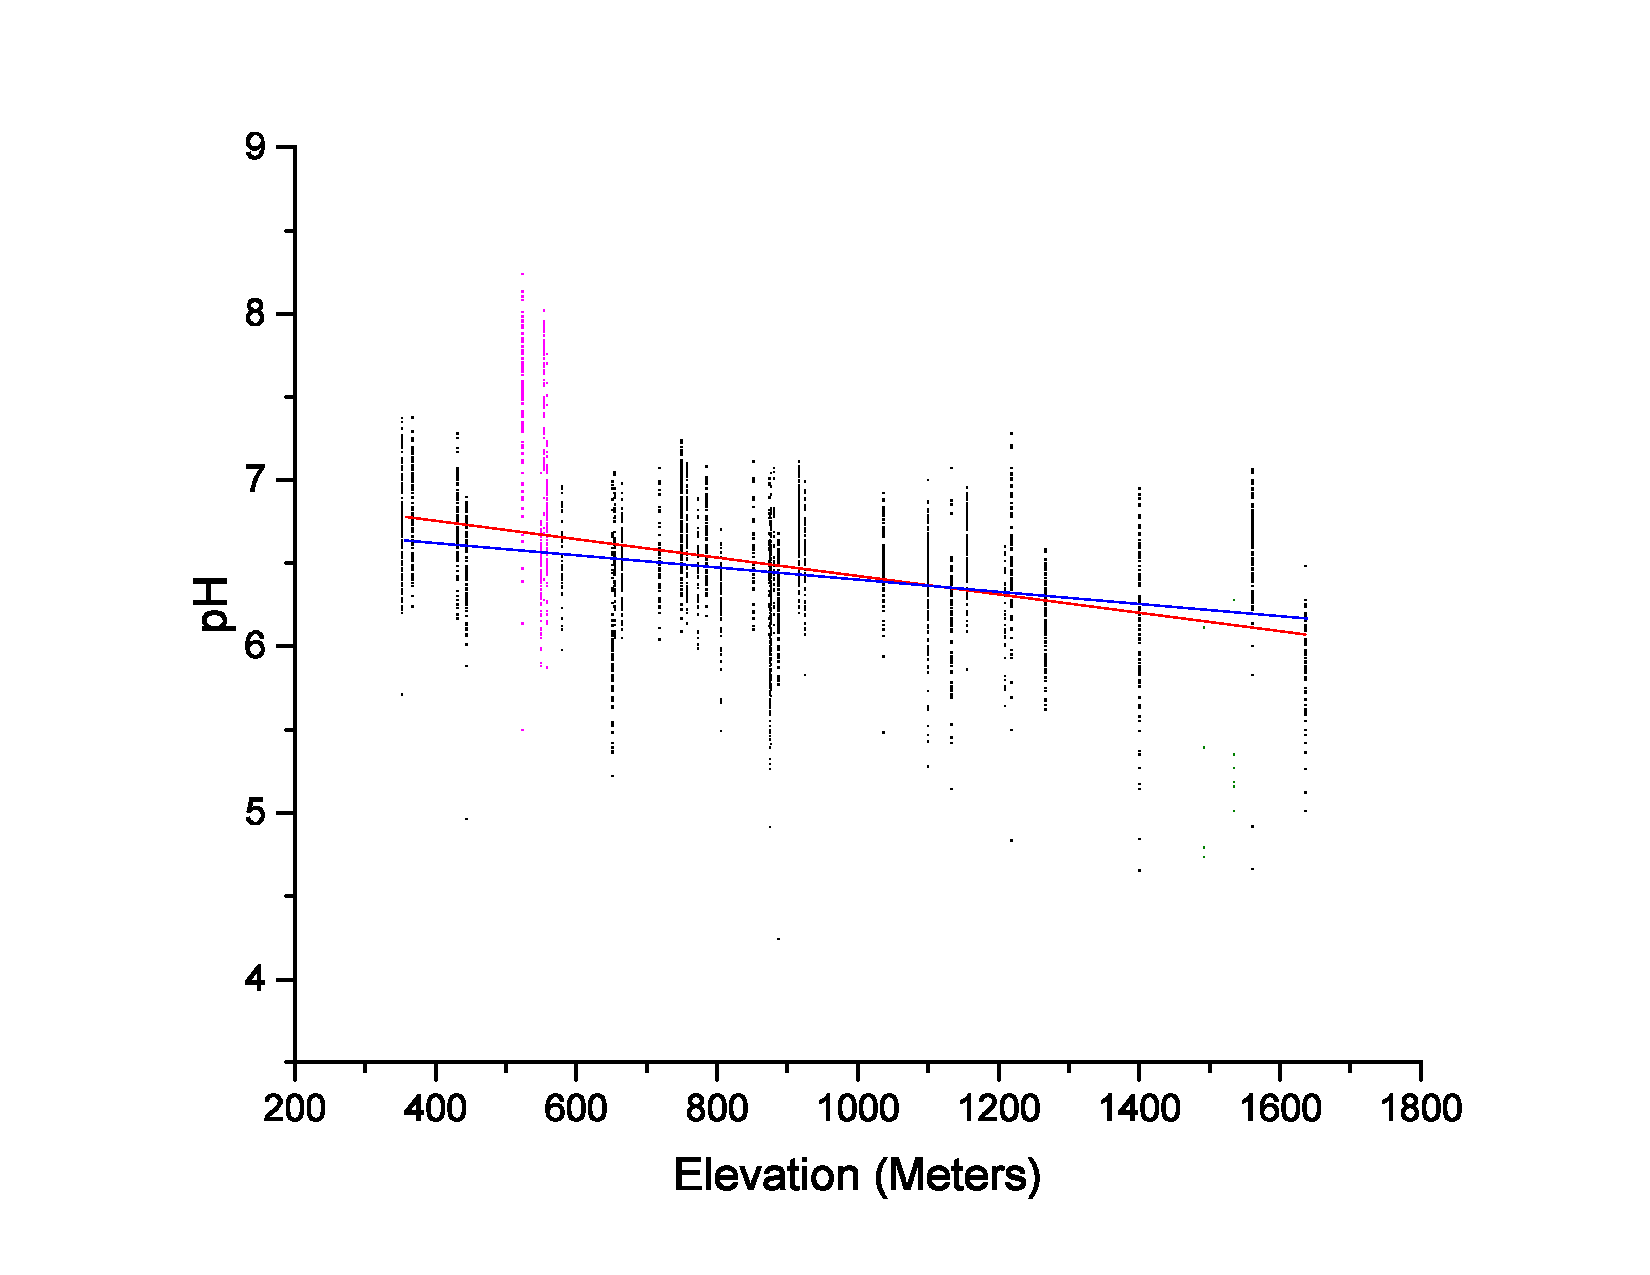
\includegraphics[width=6in]{pHdata}\\
  \caption{pH plotted vs. Elevation.  With and without outliers.}\label{fig:pHdata}
\end{figure}
\autoref{fig:pHdata} shows the pH vs. elevation plot.  It shows two trend lines, one which represents the trend of all of the data points and the other represents the trend after the influential points are removed.  Both of the trends are negative as elevation increases but the trend for all the data is steeper.  pH was plotted against the month that the sample was collected to check for seasonality.  Seasonality was expected and found for pH over one year.  The variance caused by seasonality will be removed with sine and cosine functions. 

Much of the variance in \autoref{fig:pHdata} can be attributed to known influences of the Abrams creek watershed, sites that are affected by anakeesta geology, and storm flow.  Abrams is a lower elevation, low slope area where the underlying geology is Cades Sandstone which buffers against acid rain very well.  This sandstone contributes to high ANC values which in turn keep the pH levels higher than the rest of the sites in the survey.  Site numbers 237 and 252 are sites which are down slope of road cuts that have exposed the underlying anakeesta formation  to runoff.  The anakeesta formation contains sulfidic slate which can negatively effect streams and keep their pH values very low.  
Storm flow is also usually seen as an out lier in past GRSM water quality projects.  Storms can bring high intensity rain fall which can very quickly reduce the ANC of streams.  In streams with already low ANC and pH this episodic stream acidification can be harmful to aquatic life \citep{neff2009physiological}  The lowered pH of the streams caused by the storm flow can cause leeching of the surrounding base cation minerals.  When these minerals run out, hydrogen and aluminum are released into the water.  Hydrogen will lower the pH more and aluminum is toxic to living things.  Healthy streams can rebound to normal pH values, unhealthy streams can have permanently lowered ANC due to the leaching. %check on facts of  leaching and permanently lowered ANC
 Measurements taken from storm flow can show uncharacteristically low pH values and high amounts of metals.  In this way storm flow is sometimes considered an influential group on the rest of the data, because the measurements are significantly different from the average.  Dr. Cai characterized all of the available water quality data between 1993 and 2010 as storm flow or base flow, this work is summarized in \citet{cai2012}.  Water quality data after 2010 has not been characterized.  If  all storm flow observations are to be dismissed as influential, the years 2011 and 2012 would need to be characterized.  Quick analyses were run to see how influential storm flow was on the data as a whole and it turned out that some were and many were not.  Instead of throwing out all of storm flow observations, storm flow became a reason to throw out influential observations during regression analysis.  They can be removed on a case by case basis during the regression procedure.
 
 Part of the regression procedure includes preparing the data and  identifying influential observations.  The output of a step-wise regression analysis done in SPSS can be configured to complete many different analyses in order to clean the data.  The different tests employed for this paper include tests for normality, heteroscedasticity, cook's D, DFBETAS, and DFFITS.  As observations were identified by cook's d, DFBETAS, and or DFFITS as influential they were then checked in Excel to determine why.  Modification of removal of an influential observation had to be justified or it would remain an outlier.  An example of modification of the data included a pH value that read 16.47 was changed to 6.47.  Another example is that some conductivity values were obvious copies of the ANC column which was right next to it.  These conductivity values were removed.   Some influential observations were not as obvious and if they could not be labeled as storm flow or bad data keeping they would be left in.  After sufficient attention was given to the influential observations the analysis was re-run and more influential observations could be found and attention would need be given to these also.  This process was completed for all four of the dependent variables, (pH , ANC, Nitrate, and Sulfate)
 
 The step-wise variable selection process requires a list of variables to choose from.  The original list used and the variables chosen are reported in \autoref{variables}.  The variables chosen for this list were chosen from variables available within the stream survey dataset.  The step-wise process regulates entry into the equations by the probability of the F statistic.  If this statistic was between .05 and .10 then the variable could stay.   The variables selected were used to create the fixed models in \autoref{stepwiseeq}.  If any of the time variablse were chosen by the step-wise method then the others were added.  This was done to ensure the julian date coefficient was present along with $\sin(\theta)$ and $\cos(\theta)$ for seasonality.  Many variables are present in the stream survey database but some were derived.  Mathematically seasonality can be modeled with the $\sin(\theta)$ and $\cos(\theta)$ variables as shown in \citet{helsel1992statistical}.  They represent each day of the year as a fraction of the year and place the lowest pH on January 1 and the highest on July 1.  The variables BC (base cations) represent calcium, magnesium, potassium, and sodium.  Correlations were run between each of the proposed variables  and both ANC and BC were found to be better represented as $\log_2(ANC)$ and $\log_2(BC)$.
 
 \begin{table}[htbp]
\caption{Equations created through step-wise variable selection}
\begin{tabular}{lp{7.5cm}cc}
\toprule
Dependent (n)     &Model                                                                                                                                                                                                                                                                                                                                                                                                       & Adjusted $r^2$  & Model p \\ 
\midrule
pH (3116)            &$.673\times\log_2(\text{Sum Base Cations}) + (-.368\times \text{NO}_3) + (.262\times \text{Julian Day}) + (-.266\times \text{SO}_4) + (-.050\times\cos(\theta))$                                                                                                                                       & 0.630                  & $<$0.001 \\
ANC (3116)         &$ (.415\times \text{Sum Base Cations}) + (-.185\times \text{SO}_4) + (.595\times \text{Conductivity}) + (-.102\times \text{NO}_3) + (.019\times \text{Julian Date}) + (.005\times \text{Cl}) + (.005\times \sin(\theta))$                                                & 0.984                  & 0.049 \\
NO$_3$ (3116)   &$(-.295\times \text{SO}_4) + (-3.183\times \text{ANC}) + (2.19\times \text{Conductivity}) + ( .923\times \text{Sum Base Cations}) + (.120\times \text{Julian Date}) + (.051\times \text{Cl}) + (.047\times \sin(\theta)) + (.031\times \cos(\theta))$ &0.498                   & 0.017 \\ 
SO$_4$ (3116)   &$ (-.166\times \text{NO}_3) + (2.318\times \text{Conductivity}) + (-3.229\times \text{ANC}) + (1.033\times \text{Sum Base Cations}) + (.042\times \text{Julian Date})$                                                                                                                               & 0.720                  & $<$0.001 \\ 
\bottomrule
\end{tabular}
\label{tab:stepwiseeq}
\end{table}


 The problem with these equations is still the high amount of variation within them while trying to determine a time trend.  All of the equations contain the time variables (julian date, $\sin(\theta)$, and $\cos(\theta)$ along with some other chemical variables.  Because of the difficulty of explaining what the julian date coefficient really means along side all of this other variation a second set of equations was created.  Theses equations contain only the three time variables.
 
\section{Results}

In \citet{robinson2008ph} julian date coefficients are are reported for each of the eleven historical elevation classes and across each of the dependent variables (pH, ANC, NO$_3$, and SO$_4$).  Julian date coefficients for this paper were reported in similar tables.  There are 144 different julian date coefficients in two tables.  \autoref{tab:Step-wise julian date} records the julian date coefficients calculated using equations with step-wise variables and \autoref{tab:time vars} records the julian date coefficients for  equations containing only the time variables.  Each trend line is represented by its Julian date coefficient, the $r^2$ value for the trend line, and it's statistical significance.

2 of the 72 trend lines in \autoref{tab:Step-wise julian date} are insignificant.  In contrast only 20 of the trend lines in \autoref{tab:time vars} are significant.   Insignificance is determined  by receiving a p-value greater than .05, which is the chosen $\alpha$ of the trend line.  A p-value greater than .05 rejects the hypothesis that $\beta$(the coefficient) $\neq$ 0.  A p-value greater than .05 means that there is greater than a 5$\%$ chance that $\beta$=0.  There is to much chance of no trend line for the scientific community.

\subsection{Step-wise equations}

\subsubsection{pH}

In \autoref{tab:Step-wise julian date} the julian date coefficients for pH show negative time trends in three statistically significant regression lines, all in the time range of 1993-2002.  These lines are in elevation classes 2, 3, and 5.  There is one negative trend in the third time set (2009-2012) and in the fifth elevation class but it is insignificant.   Most of the trend lines report that pH is increasing over time.

\subsubsection{ANC}

Across time sets and elevation classes trends for ANC fluctuate.  Eleven of the lines are positive and seven are negative.   Two of the three negative trends for ANC in set 2 are smaller in set 3 and one of the negative trends in set 2 becomes positive in set 3.  When comparing time set 2 to set 3 ANC trends are increasing over time. 

\subsubsection{Nitrate}

Nitrate trends in set 2 are all positive.  In set 3 nitrate has a negative trend value in elevation class 4.  The Nitrate trends for set 1 are half positive and half negative.  But from the years 2003 to 2008 all of the Nitrate slopes are positive.  In set 3 the trend in elevation class 4  have a negative slope. 

\subsubsection{Sulfate}

 Sulfate has mixed positive and negative trends for set 1 but all positive trends for set 2.   Half of the sulfate trends in set 3 are negative ( 1, 3, and 6).

\subsection{Time variables}

In \autoref{tab:time vars} only 20 of the 72 regression lines are significant, those that have acceptable p-values less than .05. 

\subsubsection{pH}

In set 1 pH has zero significant lines, set 2 and 3 combined are less than half insignificant trend lines.  The insignificance of the trend lines leaves them untrustworthy, but the trends are quite similar to those calculated in \autoref{tab:Step-wise julian date}.

\subsubsection{ANC}

There are only two significant regression lines in for ANC in \autoref{tab:time vars}.  Elevation class 5 in set 1 has a negative trend at -.148, there are no significant lines in set 2 and set 3 elevation class 5 is a positive trend at .891.  

\subsubsection{Nitrate and Sulfate}

Nitrate and sulfate both have negative trends in set 1 class 1.  These are the only negative slopes for nitrate and sulfate in \autoref{tab:time vars}, both have positive slopes in set 2 at elevation classes 1,2,4 and 6, and neither variable have significant lines in 3.
%compare to trends from robinson's paper

\subsection{Results by Comparison}

\section{Discussion}%it is interesting that the step-wise process did not choose elevation as an independent for pH

It is interesting that the step-wise process did not choose elevation or slope as an independent variable for any of the dependent variables.  \autoref{fig:pHdata} clearly shows a negative trend for pH while increasing the elevation.  %elevation is not as important as the others, elevation did not pass the .05 and .1 F probability constraints.

A trend in time is also clearly evident with a simple plot of pH and time but the mostly insignificant trends of \autoref{tab:time vars} suggest otherwise.  The three time variables alone are not enough to describe the dependent variables.

In comparing table 4 from Robinson 08 with \autoref{tab:Step-wise julian date} from this analysis it needs to be noted that the elevation classes are different and the data sets have slightly changed throughout the years.  The largest difference is the reduction of 90 sites to 43.  Abrams was not included in this analysis which would affect differences in the old elevation classes from Robinson 08 of 1,2, and 3 with elevation class 1 with this study.  The Abrams sites constantly have high outlying pH values.  Two sites (237, 252) that are in the new elevation class 6 were left out of the statistical analysis for having low outlying values.  These correspond to old elevation class 9.

One interesting comparison is between table 4 of Robinson 08 and set 1 of this analysis.  All of the pH trends presented in table 4 of Robinson 08 are negative which is what led to the findings in \citet{robinson2008ph} that pH is dropping and can drop to harmful levels in the future.  However, only half the time trend trends for set 1 for pH found in this study were negative in \autoref{tab:Step-wise julian date} and none of the trend lines for pH in \autoref{tab:time vars} are significant.  All of the rest of the pH trends for Julian date for both \autoref{tab:Step-wise julian date} and \autoref{tab:time vars} are positive when they are significant.  These differences imply that water quality was worse with 90 sites.
\begin{itemize}
	\item Why are the water quality trends trending the way they are at separate time sets ( discuss comparisons between sets in the ANOVA bonferoni section).
	\item How should the water quality variables have behaved based on known properties and \citep{robinson2008ph}.%sulfate should decline after 2008
	\item Very generally speaking these results are different than \citep{robinson2008ph} predicted.% he has a table predicting what the pH value should be.
	\item Water quality will continue to get better. % if the measurements are getting better because of pollution control
	\begin{itemize}
		\item because pollution is being regulated
	\end{itemize}
	\item there are still unknowns and prediction is still hard.
\end{itemize}
	
